\documentclass[11pt,a4paper]{article}

% --- Packages ---
\usepackage[utf8]{inputenc}
\usepackage[T1]{fontenc}
\usepackage{lmodern}
\usepackage[a4paper,top=2.2cm,bottom=2.2cm,left=2.2cm,right=2.2cm]{geometry}
\usepackage{graphicx}
\usepackage{xcolor}
\usepackage{amsmath,amssymb}
\usepackage{booktabs}
\usepackage{tabularx}
\usepackage{array}
\usepackage{enumitem}
\usepackage{titlesec}
\usepackage{fancyhdr}
\usepackage{listings}
\usepackage{float}
\usepackage{tikz}
\usetikzlibrary{shapes.geometric,arrows.meta,positioning,calc,fit}
\usepackage{caption}
\usepackage{subcaption}
\usepackage{tcolorbox}
\usepackage[colorlinks=true,linkcolor=blue!80!black,citecolor=blue!80!black,urlcolor=blue!80!black]{hyperref}

% --- Float & Layout Adjustments (Prevent Awkward Whitespaces) ---
\renewcommand{\topfraction}{0.90}
\renewcommand{\bottomfraction}{0.90}
\renewcommand{\textfraction}{0.10}
\renewcommand{\floatpagefraction}{0.80}
\setlength{\textfloatsep}{12pt plus 2pt minus 2pt}
\setlength{\intextsep}{10pt plus 2pt minus 2pt}
\setlength{\abovecaptionskip}{6pt}
\setlength{\belowcaptionskip}{4pt}

% --- Color Definitions ---
\definecolor{primaryblue}{RGB}{30, 58, 138}
\definecolor{secondaryblue}{RGB}{37, 99, 235}
\definecolor{darkslate}{RGB}{15, 23, 42}
\definecolor{lightbg}{RGB}{248, 250, 252}
\definecolor{bordercolor}{RGB}{203, 213, 225}
\definecolor{codebg}{RGB}{241, 245, 249}

% --- Section Styling ---
\titleformat{\section}
  {\normalfont\Large\bfseries\color{primaryblue}}
  {\thesection}{1em}{}[\color{primaryblue}\titlerule]
\titleformat{\subsection}
  {\normalfont\large\bfseries\color{secondaryblue}}
  {\thesubsection}{1em}{}
\titleformat{\subsubsection}
  {\normalfont\normalsize\bfseries\color{darkslate}}
  {\thesubsubsection}{1em}{}

% --- Code Listing Styling ---
\lstset{
  backgroundcolor=\color{codebg},
  basicstyle=\ttfamily\footnotesize,
  breaklines=true,
  captionpos=b,
  frame=single,
  rulecolor=\color{bordercolor},
  keywordstyle=\color{primaryblue}\bfseries,
  commentstyle=\color{gray},
  stringstyle=\color{teal},
  numbers=none,
  tabsize=2,
  showstringspaces=false
}

% --- Graphics Path ---
\graphicspath{{./}{./screenshot/}{./docs/}{./docs/screenshot/}}

\begin{document}

% =========================================================
% COVER PAGE (No Page Number)
% =========================================================
\begin{titlepage}
\thispagestyle{empty}
\begin{tikzpicture}[remember picture,overlay]
  \draw[line width=1.5pt, color=primaryblue] 
    ($(current page.north west) + (1.2cm,-1.2cm)$) 
    rectangle 
    ($(current page.south east) + (-1.2cm,1.2cm)$);
  \draw[line width=0.5pt, color=bordercolor] 
    ($(current page.north west) + (1.3cm,-1.3cm)$) 
    rectangle 
    ($(current page.south east) + (-1.3cm,1.3cm)$);
\end{tikzpicture}

\begin{center}
  \vspace*{0.2cm}
  
  % University Logo (If file exists, otherwise placeholder box handled)
  \IfFileExists{JUST_LOGO.png}{%
    
\includegraphics[height=2.2cm]{JUST_LOGO.png}\\[0.3cm]
  }{%
    \IfFileExists{docs/JUST_LOGO.png}{%
      
\includegraphics[height=2.2cm]{docs/JUST_LOGO.png}\\[0.3cm]
    }{%
      \vspace{1.8cm}
    }
  }

  {\LARGE \textbf{\textcolor{primaryblue}{JASHORE UNIVERSITY OF SCIENCE AND TECHNOLOGY}}}\\[0.2cm]
  {\large \textbf{DEPARTMENT OF COMPUTER SCIENCE AND ENGINEERING}}\\[0.2cm]
  {\normalsize \textbf{\textcolor{secondaryblue}{Course: Software Development Project-II}}}\\[0.8cm]

  \rule{0.85\textwidth}{1.2pt}\\[0.4cm]
  {\huge \textbf{Lab Report on Hotel Management System}}\\[0.3cm]
  {\Large \textbf{Project: The Haunted Hotel Management System}}\\[0.2cm]
  {\normalsize Full-Stack Web Application with ASP.NET Core (.NET 10) Clean Architecture and React 19 SPA}\\[0.3cm]
  \rule{0.85\textwidth}{1.2pt}\\[1.0cm]

  \vfill

  \begin{minipage}[t]{0.47\textwidth}
    \begin{tcolorbox}[colback=lightbg,colframe=primaryblue,arc=2mm,title=\textbf{\footnotesize SUBMITTED BY},coltitle=white,left=3mm,right=3mm,top=2mm,bottom=2mm]
      \footnotesize
      \textbf{Shafikul Islam Marwan}\\
      Student ID: \textbf{220121}\\
      Registration No: \textbf{2201020}\\
      Degree: B.Sc. in CSE\\
      Department of CSE, JUST
    \end{tcolorbox}
  \end{minipage}
  \hfill
  \begin{minipage}[t]{0.47\textwidth}
    \begin{tcolorbox}[colback=lightbg,colframe=primaryblue,arc=2mm,title=\textbf{\footnotesize SUBMITTED TO},coltitle=white,left=3mm,right=3mm,top=2mm,bottom=2mm]
      \footnotesize
      \textbf{Dr. Md. Nasim Adnan}\\
      Assistant Professor\\
      Department of CSE\\
      Jashore University of Science and Technology (JUST)
    \end{tcolorbox}
  \end{minipage}

  \vspace{0.8cm}
  {\small \textbf{Date of Submission:} 01-September-2026}
  \vspace*{0.2cm}
\end{center}
\end{titlepage}

% =========================================================
% PAGE NUMBERING STARTS ON TABLE OF CONTENTS (PAGE 1)
% =========================================================
\clearpage
\pagenumbering{arabic}
\setcounter{page}{1}

% Header and Footer setup
\pagestyle{fancy}
\fancyhf{}
\fancyhead[L]{\small \textcolor{gray}{Software Development Project-II: Hotel Management System}}
\fancyhead[R]{\small \textcolor{gray}{Shafikul Islam Marwan (220121)}}
\fancyfoot[C]{\thepage}
\renewcommand{\headrulewidth}{0.4pt}
\renewcommand{\footrulewidth}{0.4pt}

% --- Table of Contents ---
\tableofcontents
\clearpage

% =========================================================
% 1. INTRODUCTION
% =========================================================
\section{Introduction}

\subsection{Problem Statement}
In traditional hospitality operations, hotels that rely on manual record books, standalone spreadsheets, or disconnected software tools face frequent operational bottlenecks. Receptionists often encounter double-booking incidents, untracked room cleaning and maintenance states, slow customer check-in procedures, arithmetic mistakes during multi-night tariff calculations, uncoordinated shift handovers, and a lack of real-time managerial insight into occupancy and revenue figures.

The primary objective of this project is to address these operational challenges by designing and developing a centralized, secure, and responsive web-based hotel management system. The system integrates real-time room inventory management, customer registration, reservation lifecycles, payment ledger accounting, employee payroll tracking, and operational analytics into a cohesive software package.

\subsection{Case Study with Problem Identification}
\textbf{Context:} "The Haunted Hotel" is a boutique hospitality establishment comprising four distinct room tiers: Standard, Deluxe, Suite, and Penthouse. It operates a 24/7 reception desk handling direct walk-in guests, telephone reservations, billing settlements, and employee work schedules.

\textbf{Identified Operational Bottlenecks:}
\begin{itemize}[leftmargin=*]
  \item \textbf{Room State Inconsistencies:} Rooms under cleaning or maintenance are occasionally marked available on physical boards, leading to accidental guest allocation.
  \item \textbf{Fragmented Guest History:} Returning customers are registered as new records, preventing quick lookup and historical stay analysis.
  \item \textbf{Error-Prone Multi-Night Calculations:} Calculating stay durations with partial advances and custom tariffs creates accounting errors during peak hours.
  \item \textbf{Uncoordinated Shift Handovers:} Outstanding guest balances and daily cash receipts are difficult to audit across alternating front-desk shifts.
\end{itemize}

\textbf{Proposed Solution:} A full-stack web application developed with ASP.NET Core (.NET 10) following Clean Architecture, combined with a React 19 Single Page Application (SPA). The backend enforces server-calculated billing totals, automated status transitions, and strict role-based access control.

\subsection{Specification of High-Level Goals}
\begin{enumerate}[leftmargin=*]
  \item \textbf{Centralized Room Inventory:} Maintain an authoritative real-time state for every room (Available, Occupied, Under Maintenance) with defined tier rates.
  \item \textbf{Structured Booking Lifecycle:} Guide reservations strictly through sequential stages: Pending $\rightarrow$ Confirmed $\rightarrow$ Checked In $\rightarrow$ Checked Out (or Cancelled).
  \item \textbf{Server-Enforced Financial Integrity:} Guarantee that stay duration, total billing, and remaining balances are computed server-side, preventing client-side data tampering.
  \item \textbf{Operational Analytics:} Provide an executive dashboard displaying key performance indicators (KPIs), room occupancy ratios, revenue distributions, and utilization trends.
  \item \textbf{Role-Based Security:} Secure administrative operations (employee payroll and user management) while enabling efficient daily operations for staff accounts.
\end{enumerate}

% =========================================================
% 2. FEASIBILITY ANALYSIS
% =========================================================
\section{Feasibility Analysis}

\subsection{Technical Feasibility}
The system architecture was chosen based on industrial performance, reliability, and modularity:
\begin{itemize}[leftmargin=*]
  \item \textbf{Backend:} ASP.NET Core (.NET 10) Web API provides high throughput, asynchronous execution, built-in dependency injection, and clean architectural layer separation.
  \item \textbf{Frontend:} React 19 with Vite delivers a lightweight, responsive SPA with fast rendering and modular component management.
  \item \textbf{Database and ORM:} Microsoft SQL Server with Entity Framework Core 9 guarantees ACID transactional compliance, referential constraints, and automated schema migrations.
  \item \textbf{Security:} BCrypt password hashing alongside signed JWT Bearer tokens guarantees secure stateless authentication.
\end{itemize}

\subsection{Operational Feasibility}
The system aligns directly with standard front-desk workflows. Clear navigation tabs, color-coded badges, and instant toast alerts enable new front-desk operators to become productive with minimal initial orientation. All features are accessible through standard web browsers across desktop and tablet devices without requiring client-side installations.

\subsection{Economic Feasibility and Cost-Benefit Analysis}
\begin{table}[H]
\centering
\caption{Economic Feasibility and Development Tooling Cost}
\label{tab:economic_feasibility}
\begin{tabularx}{\textwidth}{l X r}
\toprule
\textbf{Category} & \textbf{Tool / Framework / Infrastructure} & \textbf{Cost (USD)} \\
\midrule
Development IDE & Visual Studio Community, VS Code, Git & \$0.00 (Open Source) \\
Runtime Frameworks & .NET 10 SDK, Node.js runtime, React 19, Vite & \$0.00 (Open Source) \\
Database Engine & Microsoft SQL Server Developer Edition & \$0.00 (Free Tier) \\
Production Hosting & VPS Deployment (2 vCPU, 4 GB RAM) & $\sim$\$15.00 / month \\
Domain \& SSL & Custom Domain with Let's Encrypt TLS & $\sim$\$12.00 / year \\
\bottomrule
\end{tabularx}
\end{table}

\noindent \textbf{Core Benefits:}
\begin{itemize}[leftmargin=*]
  \item Replaces physical ledger books, paper receipts, and manual calculation sheets.
  \item Eliminates revenue loss resulting from double booking and arithmetic errors.
  \item Reduces average check-in and checkout processing duration from 8 minutes to under 60 seconds.
\end{itemize}

\subsection{Project Schedule (SDLC Timeline)}
\begin{table}[H]
\centering
\caption{Software Development Life Cycle Phases and Deliverables}
\label{tab:gantt_table}
\begin{tabularx}{\textwidth}{l l X}
\toprule
\textbf{Phase} & \textbf{Duration} & \textbf{Key Milestones and Deliverables} \\
\midrule
Phase 1: Planning \& Requirements & Weeks 1--2 & Domain study, requirements gathering, feasibility analysis \\
Phase 2: Architectural Design & Weeks 3--5 & UML modeling, ERD construction, relational database normalization \\
Phase 3: Backend Implementation & Weeks 6--9 & Domain models, EF Core configurations, repositories, JWT auth, APIs \\
Phase 4: Frontend Development & Weeks 10--12 & React 19 SPA, dashboard analytics charts, component integration \\
Phase 5: Automated Testing & Weeks 13--14 & xUnit test suite (35 test cases), EF Core InMemory validation \\
Phase 6: Documentation \& Defense & Weeks 15--16 & Final technical report compilation, deployment verification \\
\bottomrule
\end{tabularx}
\end{table}

% =========================================================
% 3. BUSINESS REQUIREMENT ANALYSIS
% =========================================================
\section{Business Requirement Analysis}

\subsection{Information Gathering}
Interviews with front-desk staff and management revealed that manual registers created three major risks: unnoted overlapping stays, uncollected balances during checkout, and an inability to track revenue by room category over monthly periods.

\subsection{Business Processes}
The core operational flow follows six sequential stages:
\begin{enumerate}[leftmargin=*]
  \item \textbf{Inquiry:} Staff queries available rooms matching target check-in and check-out dates.
  \item \textbf{Customer Selection:} Staff selects an existing guest profile or creates a new customer record.
  \item \textbf{Reservation Initiation:} Booking is recorded with initial status \texttt{Pending}; total cost is calculated by the server.
  \item \textbf{Financial Settlement:} Staff records payment against the booking ID. Upon full payment, the booking status automatically transitions to \texttt{Confirmed}.
  \item \textbf{Check-In:} Guest arrives; status transitions to \texttt{Checked In}; room is marked unavailable.
  \item \textbf{Check-Out:} Guest departs; system validates that the outstanding balance is zero; status updates to \texttt{Checked Out}; room is marked available.
\end{enumerate}

\subsection{Stakeholder Identification and Access Matrix}
\begin{itemize}[leftmargin=*]
  \item \textbf{Administrator:} Complete system control including employee payroll management, user account provisioning, room configuration, and financial audits.
  \item \textbf{Front Desk Staff:} Operational access for customer records, room availability queries, reservation management, check-in, checkout, and payment entry.
  \item \textbf{Hotel Management:} Read-only dashboard access for monitoring key performance metrics, revenue charts, and occupancy distribution.
\end{itemize}

\subsection{Requirements Validation Matrix}
\begin{table}[H]
\centering
\caption{Requirements Validation Matrix}
\label{tab:req_matrix}
\begin{tabularx}{\textwidth}{p{4.2cm} X p{4.2cm}}
\toprule
\textbf{Business Requirement} & \textbf{System Implementation} & \textbf{Verification Method} \\
\midrule
Prevent duplicate room bookings & Date range overlap validation & \texttt{IBookingRepository.IsRoomAvailableAsync} \\
Server-enforced billing & Server-side night calculation ($\text{nights} \times \text{tariff}$) & \texttt{BookingService.CalculateTotalAmount} \\
Zero balance checkout enforcement & Outstanding balance guard check & \texttt{BookingService.CheckOutAsync} \\
Category utilization reporting & Aggregated LINQ grouping calculations & \texttt{DashboardService.GetDashboardAsync} \\
Protected payroll access & Role-based authorization policies & \texttt{[Authorize(Roles = "Admin")]} \\
\bottomrule
\end{tabularx}
\end{table}

% =========================================================
% 4. SOFTWARE REQUIREMENTS SPECIFICATION (SRS)
% =========================================================
\section{Software Requirements Specification (SRS)}

\subsection{Functional Requirements}
\begin{itemize}[leftmargin=*]
  \item \textbf{FR-1 (Authentication):} User registration and login with BCrypt password hashing and 8-hour signed JWT tokens.
  \item \textbf{FR-2 (Room Inventory):} CRUD operations for room entities with unique room numbers, category classifications, and maintenance toggles.
  \item \textbf{FR-3 (Customer Directory):} Customer profile management with unique email constraints and real-time search filtering.
  \item \textbf{FR-4 (Booking Engine):} Reservation creation with date range validation, availability checking, and server-side fee calculations.
  \item \textbf{FR-5 (Lifecycle Management):} Enforced state transitions: \texttt{Pending} $\rightarrow$ \texttt{Confirmed} $\rightarrow$ \texttt{CheckedIn} $\rightarrow$ \texttt{CheckedOut} (with cancellation support).
  \item \textbf{FR-6 (Payment Ledger):} Transaction recording with partial payment tracking, overpayment prevention, and automated confirmation promotion.
  \item \textbf{FR-7 (Employee Administration):} Staff record management with designations and monthly base salaries (restricted to Admins).
  \item \textbf{FR-8 (Analytics Dashboard):} Aggregated calculation of room counts, occupancy ratios, 6-month revenue trends, and recent transaction feeds.
\end{itemize}

\subsection{Non-Functional Requirements}
\begin{itemize}[leftmargin=*]
  \item \textbf{Performance:} API endpoints process standard read/write requests within 200 ms under typical concurrent loads.
  \item \textbf{Reliability:} Database queries run within ACID-compliant transactions with foreign key restrictions protecting audit histories.
  \item \textbf{Security:} Parameterized LINQ queries eliminate SQL injection vulnerabilities; RFC 7807 problem details mask internal database errors from API responses.
\end{itemize}

% =========================================================
% 4.3 SYSTEM MODELS AND UML DIAGRAMS
% =========================================================
\subsection{System Models and Diagrams using UML}

\subsubsection{Use Case Diagram}
The Use Case Diagram defines the operational boundary of the system, delineating actions available to Front Desk Staff and Administrators.

\begin{figure}[H]
\centering
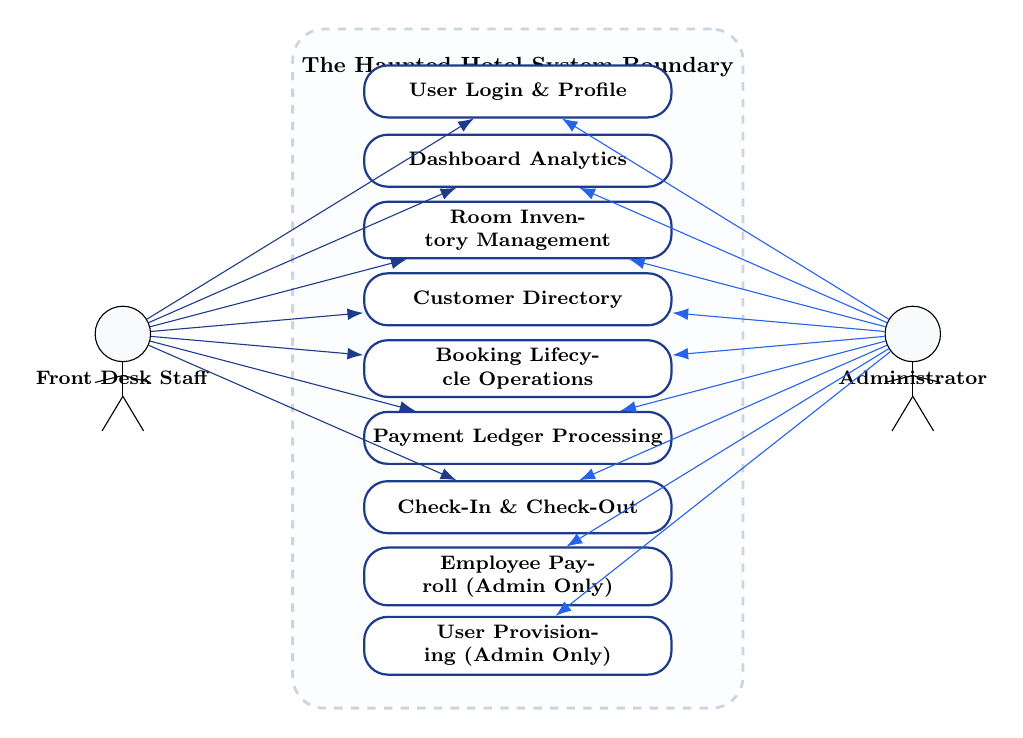
\begin{tikzpicture}[scale=0.88, transform shape,
  actor/.style={draw, circle, minimum size=0.8cm, fill=lightbg},
  usecase/.style={draw=primaryblue, fill=white, rounded corners=3mm, align=center, font=\footnotesize\bfseries, text width=4.2cm, minimum height=0.75cm, line width=0.8pt},
  sysbox/.style={draw=bordercolor, fill=lightbg!40, dashed, line width=1pt, rounded corners=4mm}
]

% System Boundary Box
\node[sysbox, minimum width=6.5cm, minimum height=9.8cm, label={[anchor=north, yshift=-3mm]\textbf{\small The Haunted Hotel System Boundary}}] (sys) at (3.5, 0) {};

% Use Cases
\node[usecase] (uc1) at (3.5, 4.0) {User Login \& Profile};
\node[usecase] (uc2) at (3.5, 3.0) {Dashboard Analytics};
\node[usecase] (uc3) at (3.5, 2.0) {Room Inventory Management};
\node[usecase] (uc4) at (3.5, 1.0) {Customer Directory};
\node[usecase] (uc5) at (3.5, 0.0) {Booking Lifecycle Operations};
\node[usecase] (uc6) at (3.5, -1.0) {Payment Ledger Processing};
\node[usecase] (uc7) at (3.5, -2.0) {Check-In \& Check-Out};
\node[usecase] (uc8) at (3.5, -3.0) {Employee Payroll (Admin Only)};
\node[usecase] (uc9) at (3.5, -4.0) {User Provisioning (Admin Only)};

% Actors
\node[actor, label=below:{\textbf{\footnotesize Front Desk Staff}}] (staff) at (-2.2, 0.5) {};
\draw (-2.2,0.1) -- (-2.2,-0.4);
\draw (-2.2,-0.1) -- (-2.6,-0.2);
\draw (-2.2,-0.1) -- (-1.8,-0.2);
\draw (-2.2,-0.4) -- (-2.5,-0.9);
\draw (-2.2,-0.4) -- (-1.9,-0.9);

\node[actor, label=below:{\textbf{\footnotesize Administrator}}] (admin) at (9.2, 0.5) {};
\draw (9.2,0.1) -- (9.2,-0.4);
\draw (9.2,-0.1) -- (8.8,-0.2);
\draw (9.2,-0.1) -- (9.6,-0.2);
\draw (9.2,-0.4) -- (8.9,-0.9);
\draw (9.2,-0.4) -- (9.5,-0.9);

% Connections - Staff
\draw[-{Latex[length=2mm]}, color=primaryblue] (staff) -- (uc1);
\draw[-{Latex[length=2mm]}, color=primaryblue] (staff) -- (uc2);
\draw[-{Latex[length=2mm]}, color=primaryblue] (staff) -- (uc3);
\draw[-{Latex[length=2mm]}, color=primaryblue] (staff) -- (uc4);
\draw[-{Latex[length=2mm]}, color=primaryblue] (staff) -- (uc5);
\draw[-{Latex[length=2mm]}, color=primaryblue] (staff) -- (uc6);
\draw[-{Latex[length=2mm]}, color=primaryblue] (staff) -- (uc7);

% Connections - Admin
\draw[-{Latex[length=2mm]}, color=secondaryblue] (admin) -- (uc1);
\draw[-{Latex[length=2mm]}, color=secondaryblue] (admin) -- (uc2);
\draw[-{Latex[length=2mm]}, color=secondaryblue] (admin) -- (uc3);
\draw[-{Latex[length=2mm]}, color=secondaryblue] (admin) -- (uc4);
\draw[-{Latex[length=2mm]}, color=secondaryblue] (admin) -- (uc5);
\draw[-{Latex[length=2mm]}, color=secondaryblue] (admin) -- (uc6);
\draw[-{Latex[length=2mm]}, color=secondaryblue] (admin) -- (uc7);
\draw[-{Latex[length=2mm]}, color=secondaryblue] (admin) -- (uc8);
\draw[-{Latex[length=2mm]}, color=secondaryblue] (admin) -- (uc9);

\end{tikzpicture}
\caption{Use Case Diagram: Operational Actors and System Boundaries}
\label{fig:use_case}
\end{figure}

\subsubsection{Class Diagram (Domain Model)}
The Class Diagram illustrates the object-oriented structure of core domain entities and their relational associations.

\begin{figure}[H]
\centering
\begin{tikzpicture}[scale=0.88, transform shape,
  entity/.style={draw=primaryblue, fill=white, rectangle, rounded corners=1.5mm, line width=0.8pt, font=\scriptsize, align=left, inner sep=2.5mm}
]

% Entities
\node[entity] (cust) at (0, 3.2) {
  \textbf{\normalsize Customer}\\[0.1cm]
  \hrule\vspace{0.1cm}
  + int Id [PK]\\
  + string FirstName\\
  + string LastName\\
  + string Email [UQ]\\
  + string Phone\\
  + string Address
};

\node[entity] (room) at (9.0, 3.2) {
  \textbf{\normalsize Room}\\[0.1cm]
  \hrule\vspace{0.1cm}
  + int Id [PK]\\
  + string RoomNumber [UQ]\\
  + string RoomType\\
  + decimal PricePerNight\\
  + bool IsAvailable
};

\node[entity] (book) at (4.5, 0) {
  \textbf{\normalsize Booking}\\[0.1cm]
  \hrule\vspace{0.1cm}
  + int Id [PK]\\
  + int CustomerId [FK]\\
  + int RoomId [FK]\\
  + DateTime CheckInDate\\
  + DateTime CheckOutDate\\
  + string Status\\
  + decimal TotalAmount
};

\node[entity] (pay) at (4.5, -3.8) {
  \textbf{\normalsize Payment}\\[0.1cm]
  \hrule\vspace{0.1cm}
  + int Id [PK]\\
  + int BookingId [FK]\\
  + decimal Amount\\
  + DateTime PaymentDate\\
  + string PaymentMethod\\
  + string PaymentStatus
};

\node[entity] (user) at (-1.5, -3.8) {
  \textbf{\normalsize User}\\[0.1cm]
  \hrule\vspace{0.1cm}
  + int Id [PK]\\
  + string Username [UQ]\\
  + string Email [UQ]\\
  + string PasswordHash\\
  + string Role
};

\node[entity] (emp) at (10.5, -3.8) {
  \textbf{\normalsize Employee}\\[0.1cm]
  \hrule\vspace{0.1cm}
  + int Id [PK]\\
  + string FirstName\\
  + string LastName\\
  + string Role\\
  + decimal Salary
};

% Relationships
\draw[-{Latex[length=2.5mm]}, line width=0.8pt] (cust) -- (book) node[midway, above left, font=\scriptsize] {1 places 0..*};
\draw[-{Latex[length=2.5mm]}, line width=0.8pt] (room) -- (book) node[midway, above right, font=\scriptsize] {1 allocated\_to 0..*};
\draw[-{Latex[length=2.5mm]}, line width=0.8pt] (book) -- (pay) node[midway, right, font=\scriptsize] {1 settled\_by 0..*};

\end{tikzpicture}
\caption{Class Diagram: Domain Entities and Relational Cardinality}
\label{fig:class_diagram}
\end{figure}

\subsubsection{Sequence Diagram: Booking Creation}
The sequence diagram models the message exchange across architectural layers when creating a new reservation.

\begin{figure}[H]
\centering
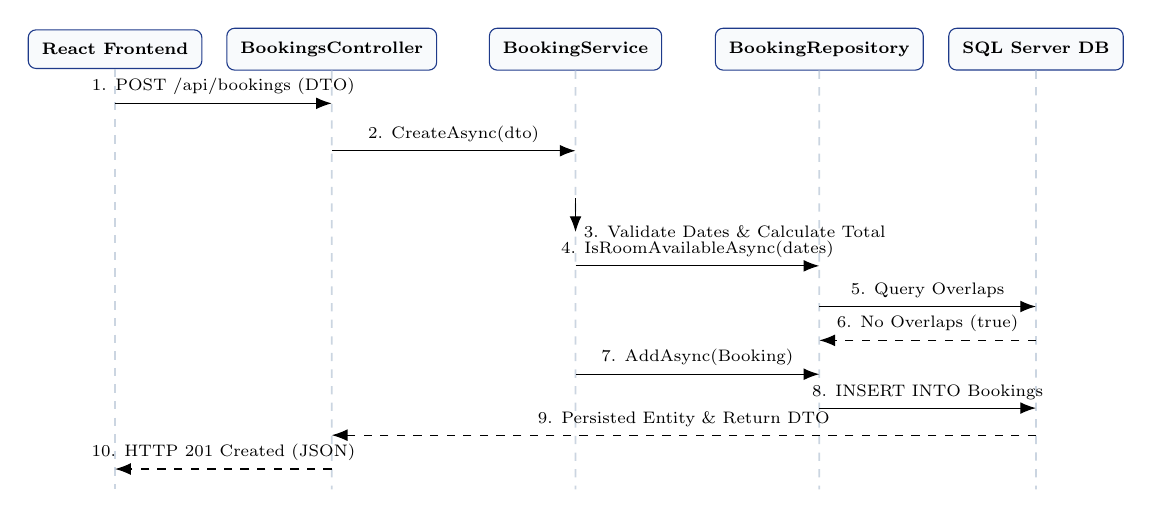
\begin{tikzpicture}[scale=0.86, transform shape,
  lifeline/.style={draw=bordercolor, dashed, line width=0.6pt},
  participant/.style={draw=primaryblue, fill=lightbg, rectangle, rounded corners=1mm, font=\scriptsize\bfseries, align=center, inner sep=2mm},
  msg/.style={-{Latex[length=2mm]}, font=\scriptsize},
  retmsg/.style={-{Latex[length=2mm]}, dashed, font=\scriptsize}
]

% Participants
\node[participant] (ui) at (0, 0) {React Frontend};
\node[participant] (ctrl) at (3.2, 0) {BookingsController};
\node[participant] (svc) at (6.8, 0) {BookingService};
\node[participant] (repo) at (10.4, 0) {BookingRepository};
\node[participant] (db) at (13.6, 0) {SQL Server DB};

% Lifelines
\draw[lifeline] (ui) -- (0, -6.5);
\draw[lifeline] (ctrl) -- (3.2, -6.5);
\draw[lifeline] (svc) -- (6.8, -6.5);
\draw[lifeline] (repo) -- (10.4, -6.5);
\draw[lifeline] (db) -- (13.6, -6.5);

% Messages
\draw[msg] (0, -0.8) -- (3.2, -0.8) node[midway, above] {1. POST /api/bookings (DTO)};
\draw[msg] (3.2, -1.5) -- (6.8, -1.5) node[midway, above] {2. CreateAsync(dto)};
\draw[msg] (6.8, -2.2) -- (6.8, -2.7) node[right, align=left] {3. Validate Dates \& Calculate Total};
\draw[msg] (6.8, -3.2) -- (10.4, -3.2) node[midway, above] {4. IsRoomAvailableAsync(dates)};
\draw[msg] (10.4, -3.8) -- (13.6, -3.8) node[midway, above] {5. Query Overlaps};
\draw[retmsg] (13.6, -4.3) -- (10.4, -4.3) node[midway, above] {6. No Overlaps (true)};
\draw[msg] (6.8, -4.8) -- (10.4, -4.8) node[midway, above] {7. AddAsync(Booking)};
\draw[msg] (10.4, -5.3) -- (13.6, -5.3) node[midway, above] {8. INSERT INTO Bookings};
\draw[retmsg] (13.6, -5.7) -- (3.2, -5.7) node[midway, above] {9. Persisted Entity \& Return DTO};
\draw[retmsg] (3.2, -6.2) -- (0, -6.2) node[midway, above] {10. HTTP 201 Created (JSON)};

\end{tikzpicture}
\caption{Sequence Diagram: Reservation Creation and Availability Verification}
\label{fig:seq_booking}
\end{figure}

\subsubsection{Activity Diagram: Guest Lifecycle}
The Activity Diagram details the end-to-end guest journey through room reservation, check-in, stay, and checkout settlement.

\begin{figure}[H]
\centering
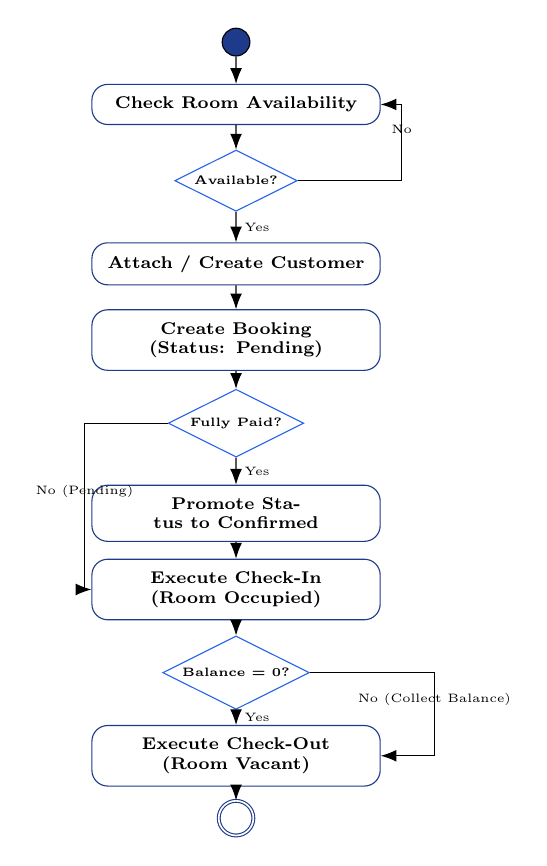
\begin{tikzpicture}[scale=0.88, transform shape,
  startnode/.style={draw, circle, fill=primaryblue, minimum size=0.4cm},
  endnode/.style={draw=primaryblue, double, circle, fill=white, minimum size=0.5cm},
  action/.style={draw=primaryblue, fill=white, rectangle, rounded corners=2mm, font=\scriptsize\bfseries, align=center, text width=3.8cm, inner sep=1.8mm},
  decision/.style={draw=secondaryblue, diamond, aspect=2, font=\tiny\bfseries, align=center, inner sep=1.5pt},
  flow/.style={-{Latex[length=2mm]}, font=\tiny}
]

\node[startnode] (start) at (0, 0) {};
\node[action] (inq) at (0, -0.9) {Check Room Availability};
\node[decision] (d1) at (0, -2.0) {Available?};
\node[action] (reg) at (0, -3.2) {Attach / Create Customer};
\node[action] (book) at (0, -4.3) {Create Booking (Status: Pending)};
\node[decision] (d2) at (0, -5.5) {Fully Paid?};
\node[action] (conf) at (0, -6.8) {Promote Status to Confirmed};
\node[action] (checkin) at (0, -7.9) {Execute Check-In (Room Occupied)};
\node[decision] (d3) at (0, -9.1) {Balance = 0?};
\node[action] (checkout) at (0, -10.3) {Execute Check-Out (Room Vacant)};
\node[endnode] (finish) at (0, -11.2) {};

% Connections
\draw[flow] (start) -- (inq);
\draw[flow] (inq) -- (d1);
\draw[flow] (d1) -- node[right] {Yes} (reg);
\draw[flow] (d1.east) -- ++(1.5,0) |- node[near start, above] {No} (inq.east);
\draw[flow] (reg) -- (book);
\draw[flow] (book) -- (d2);
\draw[flow] (d2) -- node[right] {Yes} (conf);
\draw[flow] (d2.west) -- ++(-1.2,0) |- node[near start, above] {No (Pending)} (checkin.west);
\draw[flow] (conf) -- (checkin);
\draw[flow] (checkin) -- (d3);
\draw[flow] (d3) -- node[right] {Yes} (checkout);
\draw[flow] (d3.east) -- ++(1.8,0) |- node[near start, above] {No (Collect Balance)} (checkout.east);
\draw[flow] (checkout) -- (finish);

\end{tikzpicture}
\caption{Activity Diagram: Guest Lifecycle and Status Transitions}
\label{fig:act_diagram}
\end{figure}

\subsubsection{Data Flow Diagrams (Level 0 and Level 1)}
The Context Diagram (Level 0) models the interactions between the system and its external stakeholders.

\begin{figure}[H]
\centering
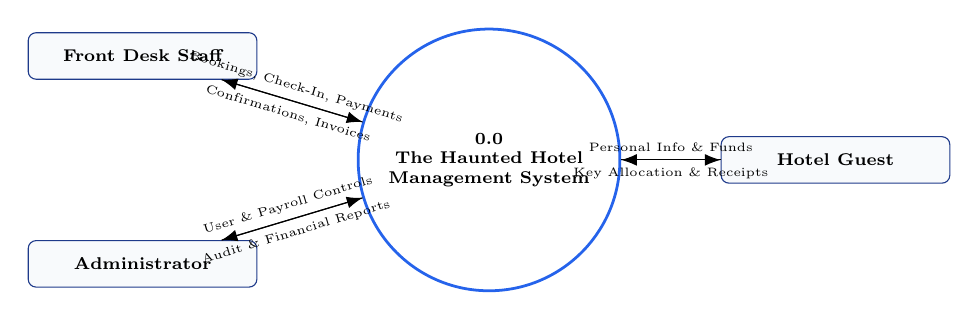
\begin{tikzpicture}[scale=0.88, transform shape,
  entity/.style={draw=primaryblue, fill=lightbg, rectangle, rounded corners=1mm, font=\scriptsize\bfseries, align=center, inner sep=2.5mm, text width=2.8cm},
  process/.style={draw=secondaryblue, fill=white, circle, font=\scriptsize\bfseries, align=center, inner sep=2mm, text width=3.2cm, line width=1pt},
  flow/.style={-{Latex[length=2mm]}, font=\tiny}
]

\node[process] (sys) at (0, 0) {0.0\\The Haunted Hotel\\Management System};
\node[entity] (staff) at (-5.0, 1.5) {Front Desk Staff};
\node[entity] (admin) at (-5.0, -1.5) {Administrator};
\node[entity] (guest) at (5.0, 0) {Hotel Guest};

\draw[flow] (staff) -- node[above, sloped] {Bookings, Check-In, Payments} (sys);
\draw[flow] (sys) -- node[below, sloped] {Confirmations, Invoices} (staff);
\draw[flow] (admin) -- node[above, sloped] {User \& Payroll Controls} (sys);
\draw[flow] (sys) -- node[below, sloped] {Audit \& Financial Reports} (admin);
\draw[flow] (guest) -- node[above, sloped] {Personal Info \& Funds} (sys);
\draw[flow] (sys) -- node[below, sloped] {Key Allocation \& Receipts} (guest);

\end{tikzpicture}
\caption{Data Flow Diagram: Level 0 Context Model}
\label{fig:dfd_level0}
\end{figure}

% =========================================================
% 4.3.7 RELATIONAL DATABASE SCHEMA
% =========================================================
\subsubsection{Relational Database Schema Specifications}

\begin{table}[H]
\centering
\caption{Relational Database Schema Specifications}
\label{tab:db_schema}
\begin{tabularx}{\textwidth}{l l l X}
\toprule
\textbf{Column Name} & \textbf{Data Type} & \textbf{Constraint} & \textbf{Description} \\
\midrule
\multicolumn{4}{l}{\textbf{Table: Users (Authentication and Roles)}} \\
\texttt{Id} & \texttt{INT} & PK, IDENTITY & Unique user identifier \\
\texttt{Username} & \texttt{NVARCHAR(100)} & NOT NULL, UQ & System login handle \\
\texttt{Email} & \texttt{NVARCHAR(150)} & NOT NULL, UQ & User email address \\
\texttt{PasswordHash} & \texttt{NVARCHAR(MAX)} & NOT NULL & BCrypt password hash \\
\texttt{Role} & \texttt{NVARCHAR(50)} & NOT NULL & Access role (Admin, Staff) \\
\midrule
\multicolumn{4}{l}{\textbf{Table: Customers (Guest Master Records)}} \\
\texttt{Id} & \texttt{INT} & PK, IDENTITY & Unique customer record ID \\
\texttt{FirstName} & \texttt{NVARCHAR(100)} & NOT NULL & Guest given name \\
\texttt{LastName} & \texttt{NVARCHAR(100)} & NOT NULL & Guest family name \\
\texttt{Email} & \texttt{NVARCHAR(150)} & NOT NULL, UQ & Guest contact email \\
\texttt{Phone} & \texttt{NVARCHAR(20)} & NOT NULL & Contact phone number \\
\midrule
\multicolumn{4}{l}{\textbf{Table: Rooms (Room Inventory)}} \\
\texttt{Id} & \texttt{INT} & PK, IDENTITY & Unique room identifier \\
\texttt{RoomNumber} & \texttt{NVARCHAR(20)} & NOT NULL, UQ & Room designator (e.g., 101, 201) \\
\texttt{RoomType} & \texttt{NVARCHAR(50)} & NOT NULL & Tier (Standard, Deluxe, Suite, Penthouse) \\
\texttt{PricePerNight} & \texttt{DECIMAL(18,2)} & NOT NULL & Nightly stay tariff \\
\texttt{IsAvailable} & \texttt{BIT} & NOT NULL & Operational status (1 = Available, 0 = Off) \\
\midrule
\multicolumn{4}{l}{\textbf{Table: Bookings (Reservation Records)}} \\
\texttt{Id} & \texttt{INT} & PK, IDENTITY & Unique reservation ID \\
\texttt{CustomerId} & \texttt{INT} & FK $\rightarrow$ Customers & Reference to guest entity \\
\texttt{RoomId} & \texttt{INT} & FK $\rightarrow$ Rooms & Reference to allocated room \\
\texttt{CheckInDate} & \texttt{DATETIME2} & NOT NULL & Scheduled check-in date \\
\texttt{CheckOutDate} & \texttt{DATETIME2} & NOT NULL & Scheduled check-out date \\
\texttt{Status} & \texttt{NVARCHAR(50)} & NOT NULL & State (Pending, Confirmed, CheckedIn, etc.) \\
\texttt{TotalAmount} & \texttt{DECIMAL(18,2)} & NOT NULL & Computed total booking fee \\
\midrule
\multicolumn{4}{l}{\textbf{Table: Payments (Financial Ledger)}} \\
\texttt{Id} & \texttt{INT} & PK, IDENTITY & Transaction record ID \\
\texttt{BookingId} & \texttt{INT} & FK $\rightarrow$ Bookings & Associated reservation ID \\
\texttt{Amount} & \texttt{DECIMAL(18,2)} & NOT NULL & Paid transaction value \\
\texttt{PaymentMethod} & \texttt{NVARCHAR(50)} & NOT NULL & Method (Cash, Card, Bank Transfer) \\
\texttt{PaymentStatus} & \texttt{NVARCHAR(50)} & NOT NULL & Status (Paid, Pending, Failed) \\
\bottomrule
\end{tabularx}
\end{table}

% =========================================================
% 5. SOFTWARE DEVELOPMENT
% =========================================================
\section{Software Development}

\subsection{Backend Architectural Design (Clean Architecture)}
The backend adheres strictly to Clean Architecture principles across four independent projects:
\begin{enumerate}[leftmargin=*]
  \item \textbf{\texttt{HotelManagement.Domain}:} Core enterprise entities (\texttt{Room}, \texttt{Customer}, \texttt{Booking}, \texttt{Payment}, \texttt{Employee}, \texttt{User}) with zero external dependencies.
  \item \textbf{\texttt{HotelManagement.Application}:} Service contracts (\texttt{IBookingService}, \texttt{IRoomService}), repository interfaces, DTOs, and business logic execution.
  \item \textbf{\texttt{HotelManagement.Infrastructure}:} Data persistence via Entity Framework Core 9, \texttt{HotelDbContext}, repository implementations, and database migrations.
  \item \textbf{\texttt{HotelManagement.API}:} Presentation layer exposing RESTful controller endpoints, JWT authentication middleware, and Swagger documentation.
\end{enumerate}

\subsection{Categorized RESTful API Endpoints}
\begin{table}[H]
\centering
\caption{Key RESTful API Endpoints and Authorization Policies}
\label{tab:api_endpoints}
\begin{tabularx}{\textwidth}{l l l X}
\toprule
\textbf{HTTP} & \textbf{Endpoint Route} & \textbf{Access} & \textbf{Functional Description} \\
\midrule
\texttt{POST} & \texttt{/api/auth/register} & Public & Register a new user account \\
\texttt{POST} & \texttt{/api/auth/login} & Public & Authenticate user and issue JWT token \\
\texttt{GET} & \texttt{/api/dashboard} & Staff, Admin & Retrieve aggregated statistics and chart data \\
\texttt{GET} & \texttt{/api/rooms/available} & Staff, Admin & Query available rooms for target date range \\
\texttt{POST} & \texttt{/api/rooms} & Admin & Add a new room into inventory \\
\texttt{POST} & \texttt{/api/bookings} & Staff, Admin & Create booking with server-calculated tariff \\
\texttt{PATCH} & \texttt{/api/bookings/\{id\}/check-in} & Staff, Admin & Check in guest (marks room occupied) \\
\texttt{PATCH} & \texttt{/api/bookings/\{id\}/check-out} & Staff, Admin & Check out guest (enforces zero balance) \\
\texttt{POST} & \texttt{/api/payments} & Staff, Admin & Record payment (auto-confirms if fully paid) \\
\texttt{GET} & \texttt{/api/employees} & Admin & List staff payroll records and salaries \\
\bottomrule
\end{tabularx}
\end{table}

\subsection{Global Exception Handling}
The backend registers an \texttt{IExceptionHandler} implementation (\texttt{GlobalExceptionHandler}) in \texttt{Program.cs} to catch unhandled errors and format them according to the RFC 7807 ProblemDetails specification. Unique constraint violations (such as duplicate emails or room numbers) return HTTP 409 Conflict, validation failures return HTTP 400 Bad Request, and unauthorized access returns HTTP 401 Unauthorized, while internal stack traces are withheld from production clients.

% =========================================================
% 5.6 USER INTERFACE IMPLEMENTATIONS (SCREENSHOTS)
% =========================================================
\subsection{User Interface Implementations and Screenshots}

\begin{figure}[H]
\centering
\IfFileExists{Registration.png}{%
  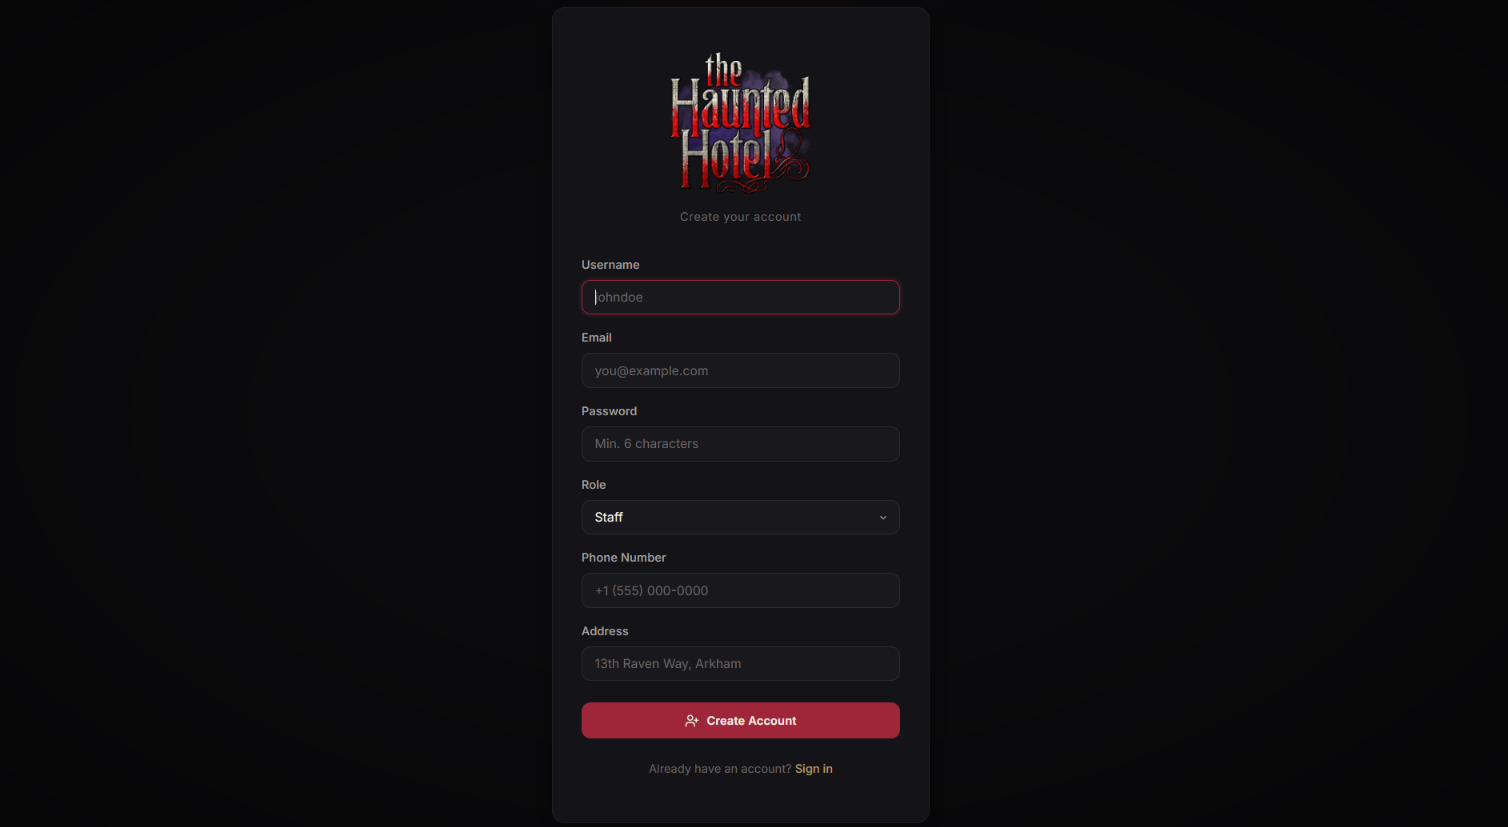
\includegraphics[width=0.92\textwidth]{Registration.png}
}{%
  \IfFileExists{docs/screenshot/Registration.png}{%
    
\includegraphics[width=0.92\textwidth]{docs/screenshot/Registration.png}
  }{%
    \fbox{\parbox{0.9\textwidth}{\centering \vspace{2cm} [Screenshot: User Registration Screen] \vspace{2cm}}}
  }
}
\caption{User Registration Interface: Secure Account Provisioning with Role Selection}
\label{fig:ui_reg}
\end{figure}

\begin{figure}[H]
\centering
\IfFileExists{Login.png}{%
  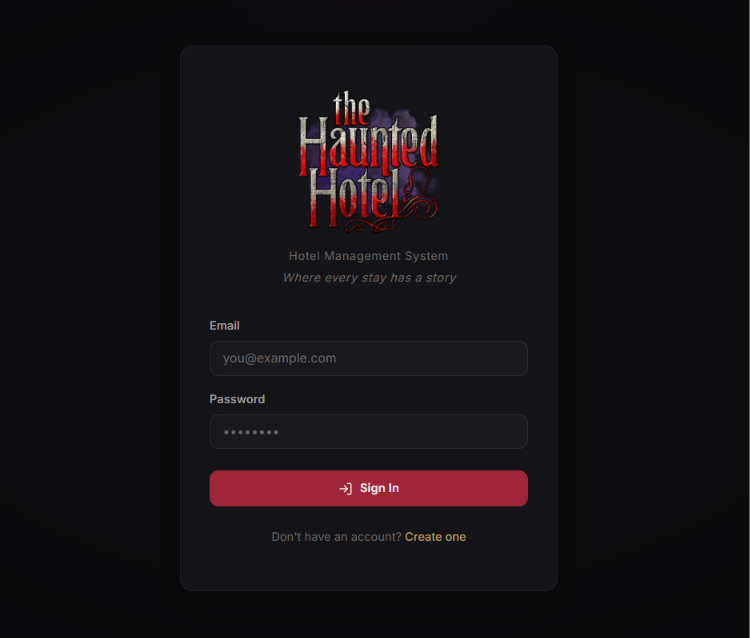
\includegraphics[width=0.92\textwidth]{Login.png}
}{%
  \IfFileExists{docs/screenshot/Login.png}{%
    
\includegraphics[width=0.92\textwidth]{docs/screenshot/Login.png}
  }{%
    \fbox{\parbox{0.9\textwidth}{\centering \vspace{2cm} [Screenshot: User Login Screen] \vspace{2cm}}}
  }
}
\caption{User Login Interface: JWT Authentication and Credential Validation}
\label{fig:ui_login}
\end{figure}

\begin{figure}[H]
\centering
\IfFileExists{Dashboard.png}{%
  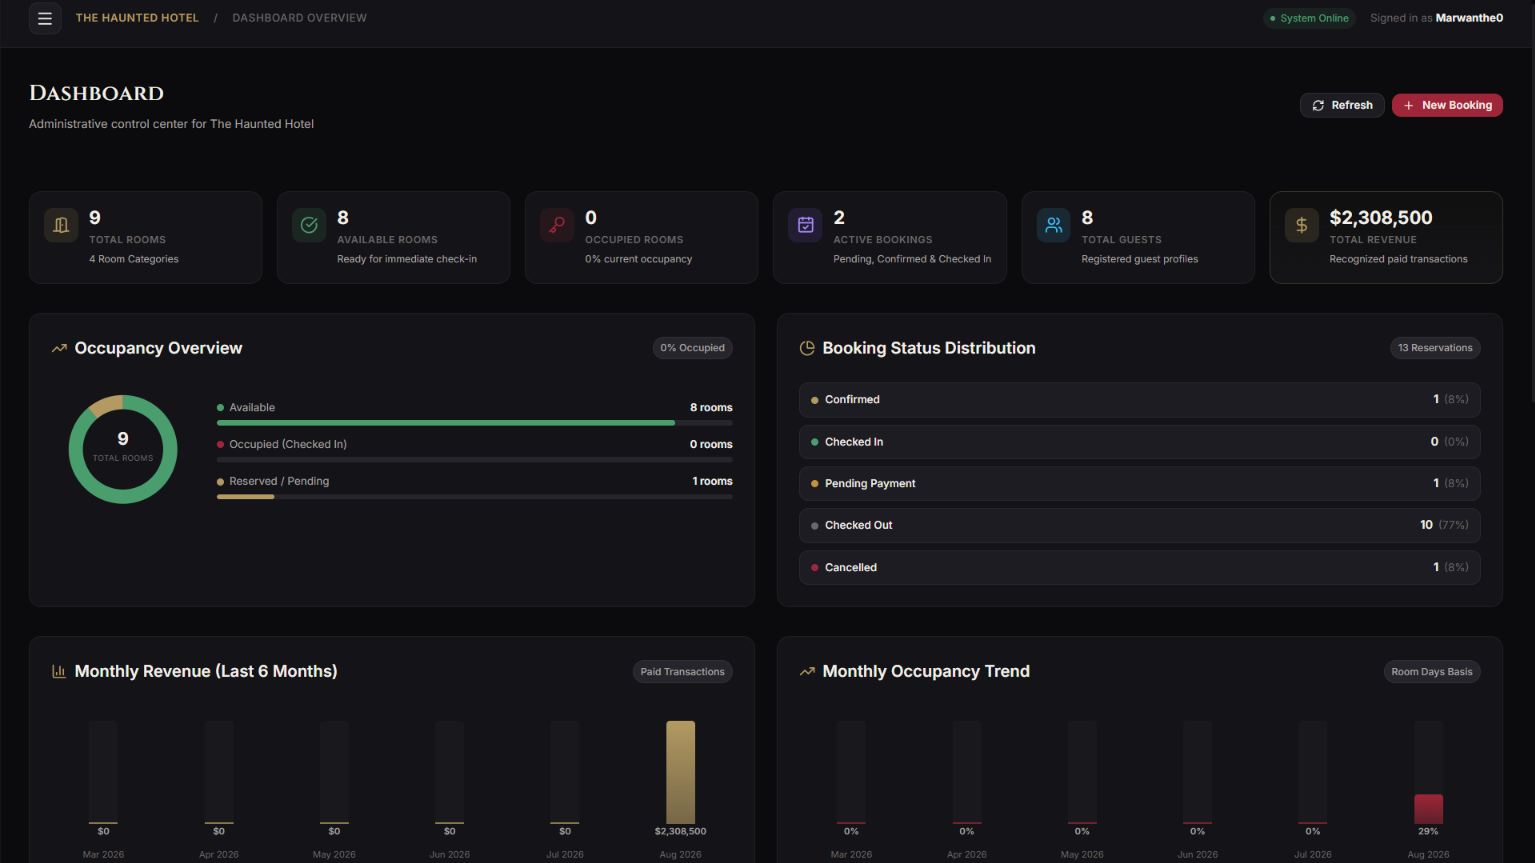
\includegraphics[width=0.92\textwidth]{Dashboard.png}
}{%
  \IfFileExists{docs/screenshot/Dashboard.png}{%
    
\includegraphics[width=0.92\textwidth]{docs/screenshot/Dashboard.png}
  }{%
    \fbox{\parbox{0.9\textwidth}{\centering \vspace{2cm} [Screenshot: Executive Dashboard Top Section] \vspace{2cm}}}
  }
}
\caption{Executive Dashboard: KPI Summary Cards, Occupancy Donut, and Revenue Trends}
\label{fig:ui_dash1}
\end{figure}

\begin{figure}[H]
\centering
\IfFileExists{Dashboard2.png}{%
  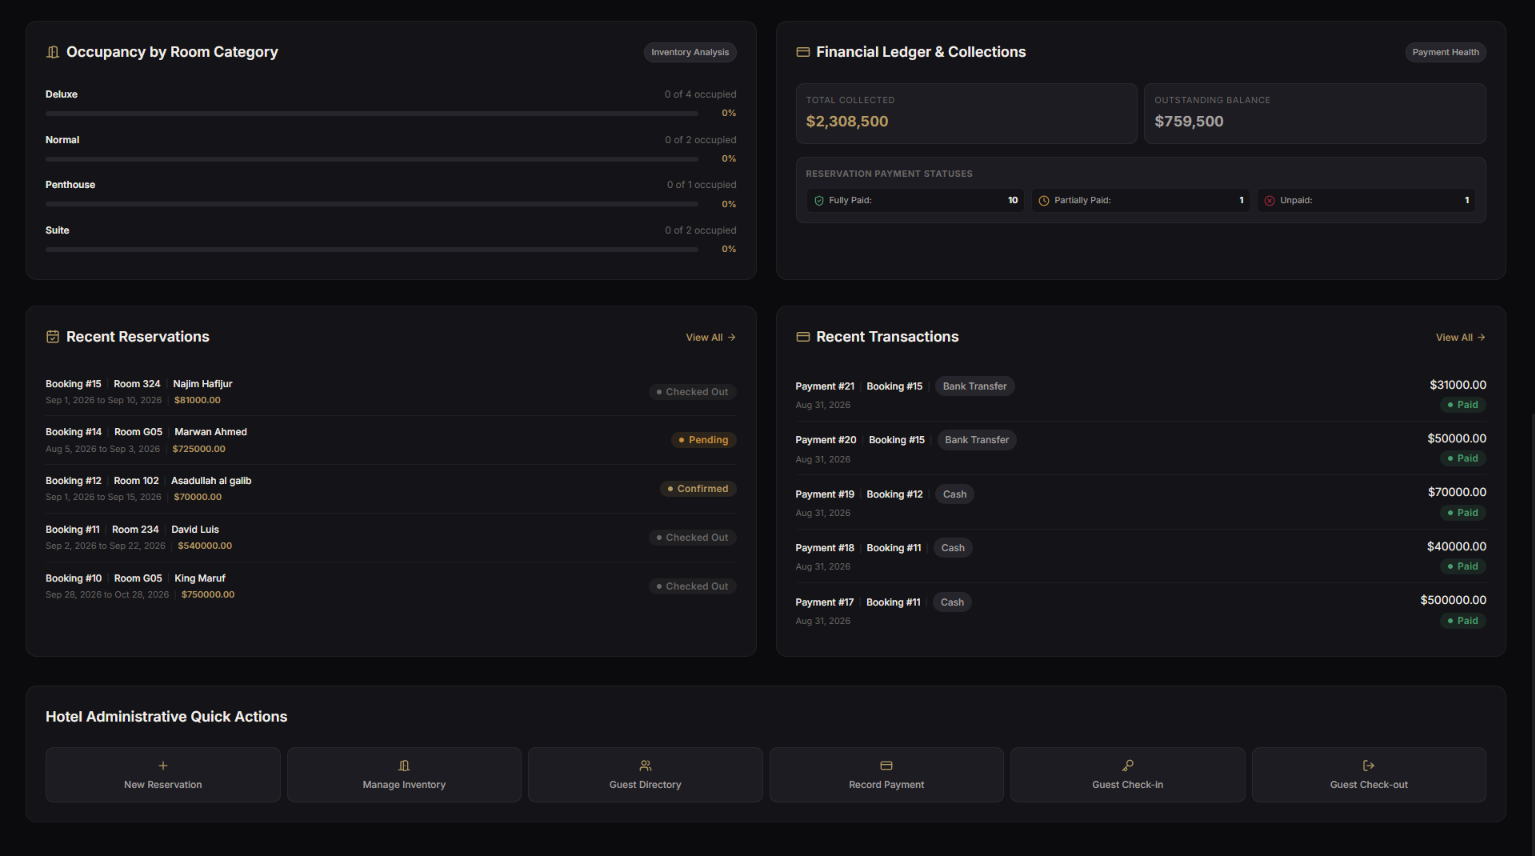
\includegraphics[width=0.92\textwidth]{Dashboard2.png}
}{%
  \IfFileExists{docs/screenshot/Dashboard2.png}{%
    
\includegraphics[width=0.92\textwidth]{docs/screenshot/Dashboard2.png}
  }{%
    \fbox{\parbox{0.9\textwidth}{\centering \vspace{2cm} [Screenshot: Executive Dashboard Bottom Section] \vspace{2cm}}}
  }
}
\caption{Executive Dashboard: Category Utilization, Financial Ledger, and Action Shortcuts}
\label{fig:ui_dash2}
\end{figure}

\begin{figure}[H]
\centering
\IfFileExists{Room_Management.png}{%
  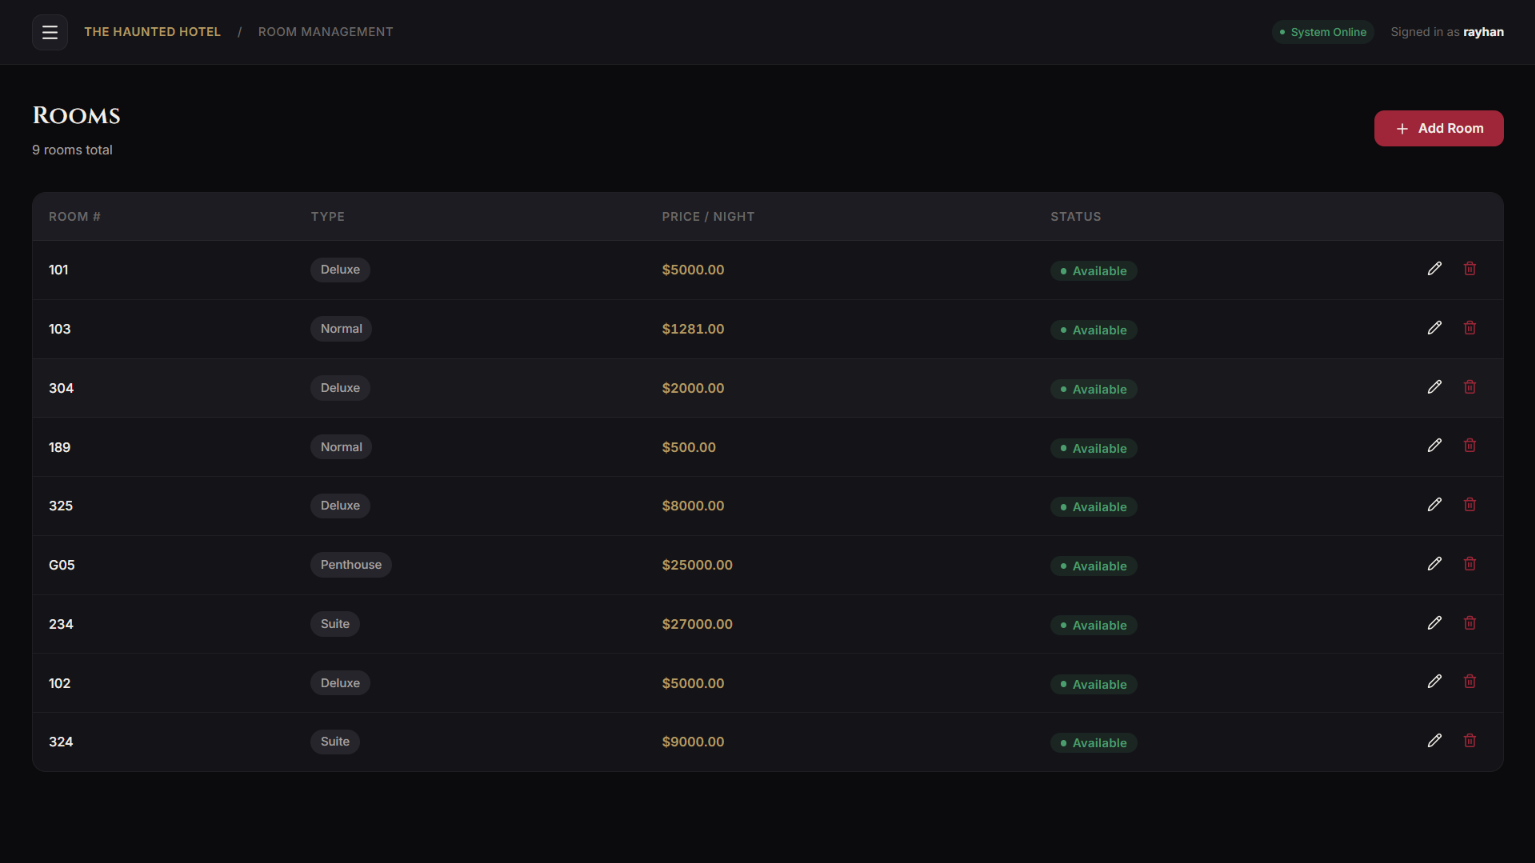
\includegraphics[width=0.92\textwidth]{Room_Management.png}
}{%
  \IfFileExists{docs/screenshot/Room_Management.png}{%
    
\includegraphics[width=0.92\textwidth]{docs/screenshot/Room_Management.png}
  }{%
    \fbox{\parbox{0.9\textwidth}{\centering \vspace{2cm} [Screenshot: Room Management Interface] \vspace{2cm}}}
  }
}
\caption{Room Inventory View: Room Allocation, Tariffs, and Maintenance Status}
\label{fig:ui_room}
\end{figure}

\begin{figure}[H]
\centering
\IfFileExists{Booking_Management.png}{%
  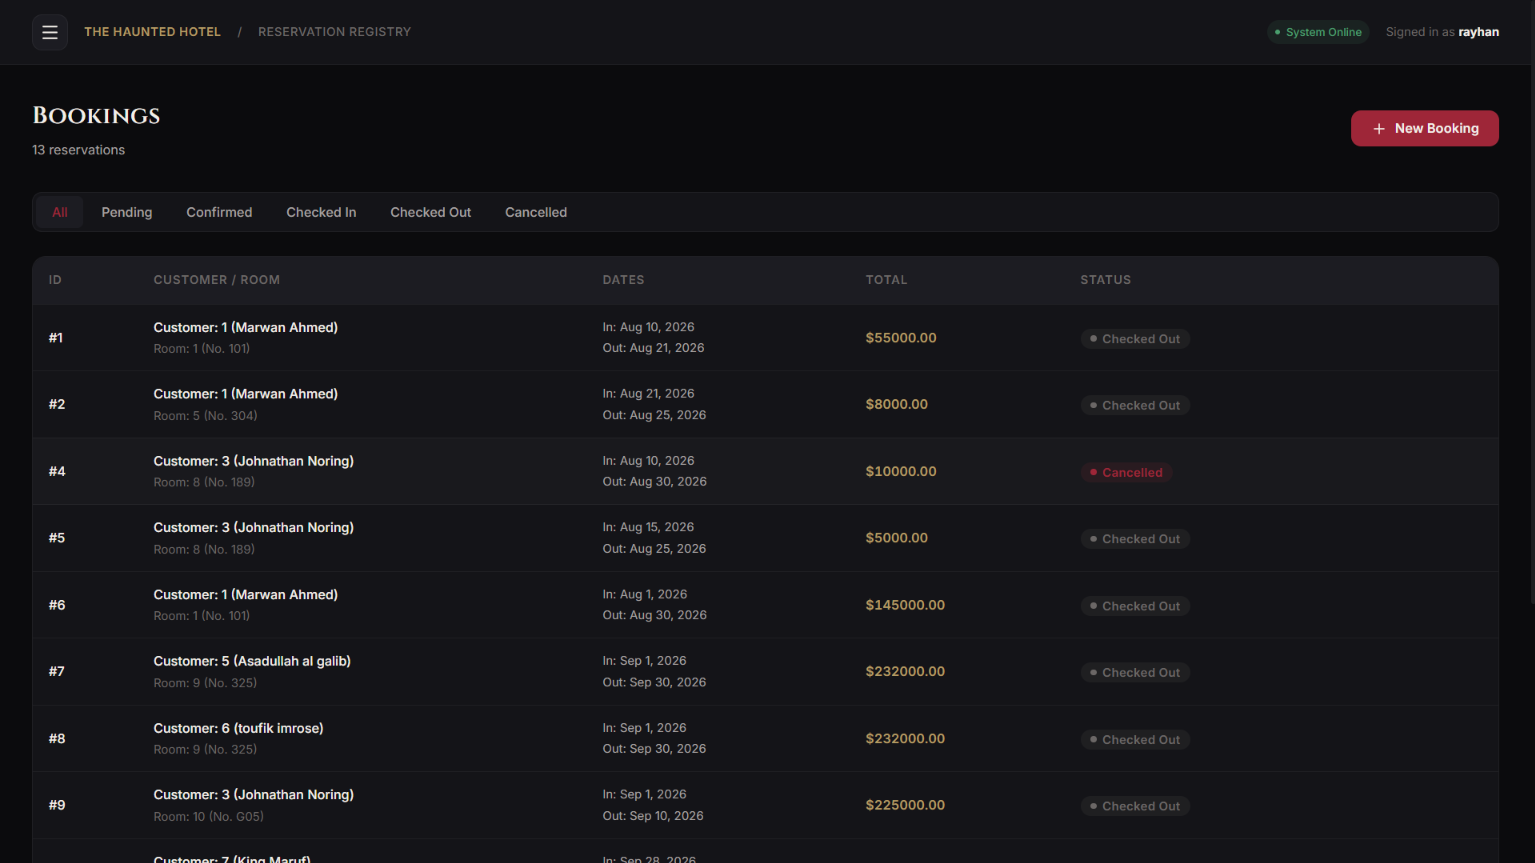
\includegraphics[width=0.92\textwidth]{Booking_Management.png}
}{%
  \IfFileExists{docs/screenshot/Booking_Management.png}{%
    
\includegraphics[width=0.92\textwidth]{docs/screenshot/Booking_Management.png}
  }{%
    \fbox{\parbox{0.9\textwidth}{\centering \vspace{2cm} [Screenshot: Booking Management Interface] \vspace{2cm}}}
  }
}
\caption{Booking Management View: Reservation Filtering, Check-In, and Checkout Controls}
\label{fig:ui_booking}
\end{figure}

\begin{figure}[H]
\centering
\IfFileExists{Customer_Management.png}{%
  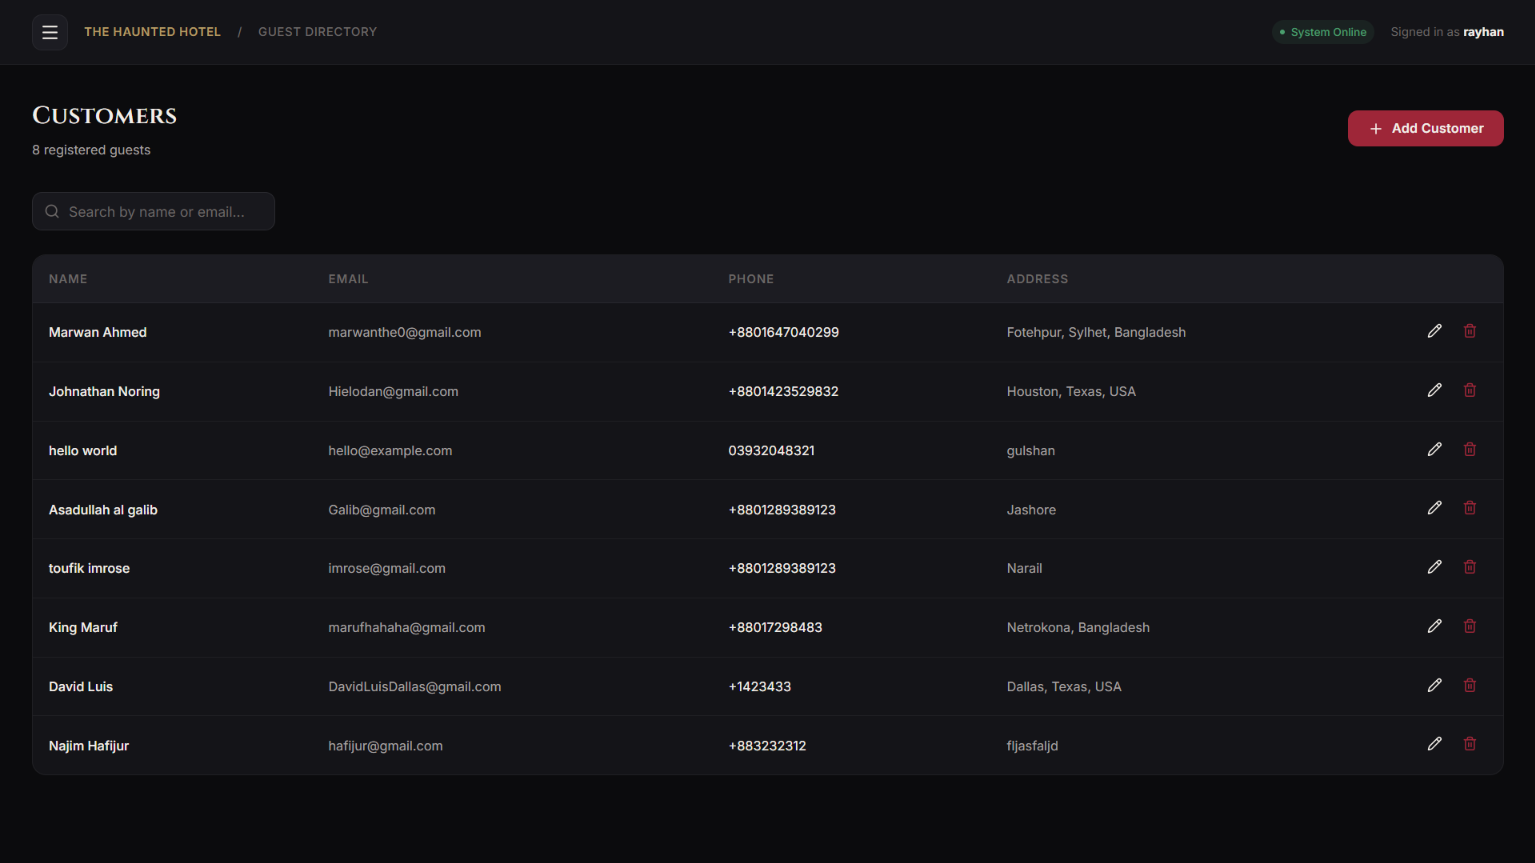
\includegraphics[width=0.92\textwidth]{Customer_Management.png}
}{%
  \IfFileExists{docs/screenshot/Customer_Management.png}{%
    
\includegraphics[width=0.92\textwidth]{docs/screenshot/Customer_Management.png}
  }{%
    \fbox{\parbox{0.9\textwidth}{\centering \vspace{2cm} [Screenshot: Customer Directory Interface] \vspace{2cm}}}
  }
}
\caption{Customer Directory View: Guest Profile Records and Real-Time Search}
\label{fig:ui_cust}
\end{figure}

\begin{figure}[H]
\centering
\IfFileExists{Payment_Management.png}{%
  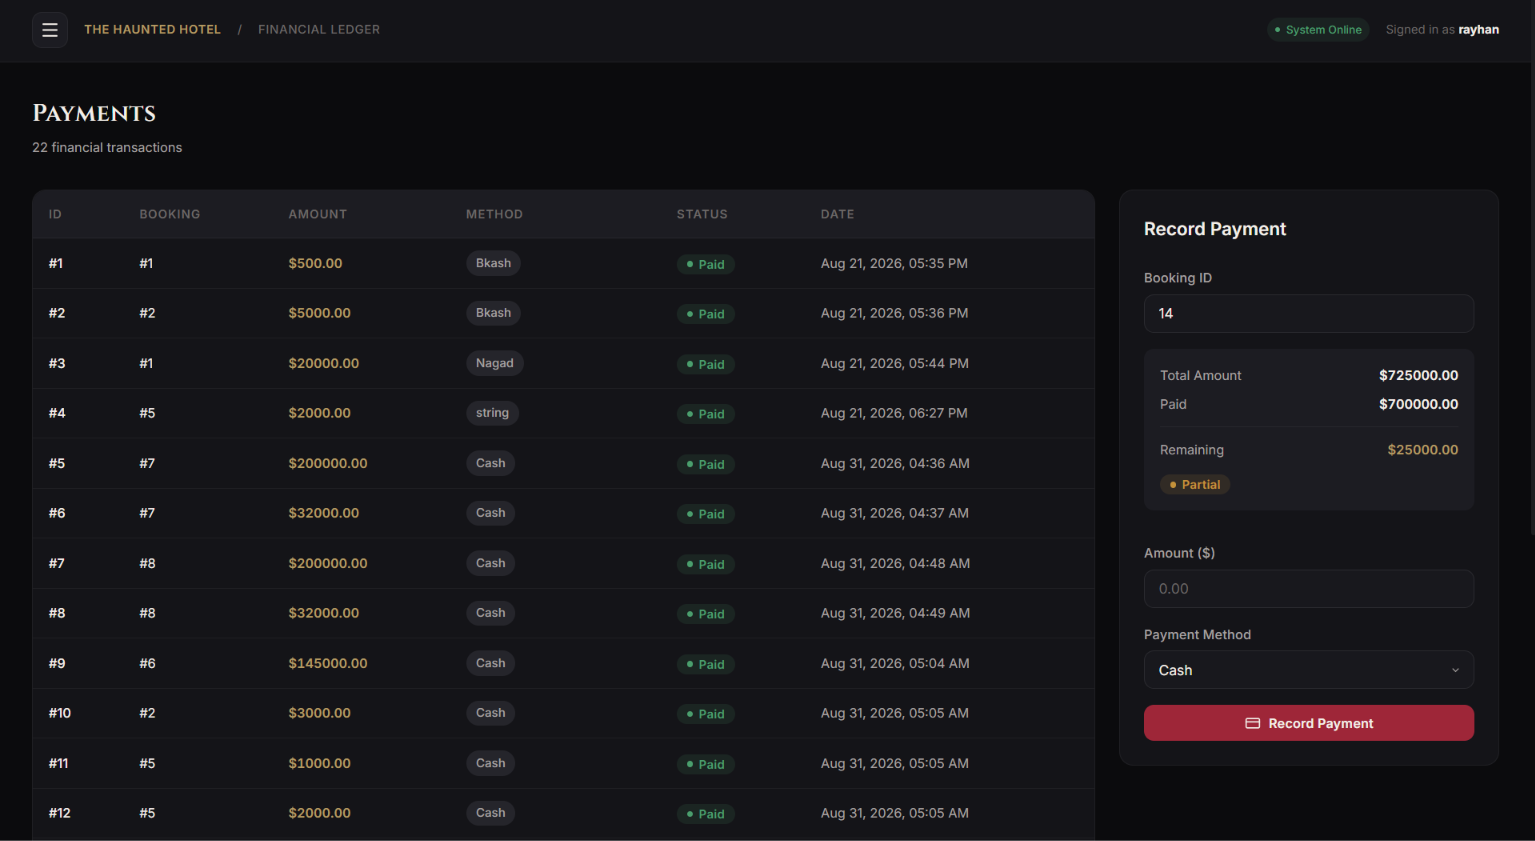
\includegraphics[width=0.92\textwidth]{Payment_Management.png}
}{%
  \IfFileExists{docs/screenshot/Payment_Management.png}{%
    
\includegraphics[width=0.92\textwidth]{docs/screenshot/Payment_Management.png}
  }{%
    \fbox{\parbox{0.9\textwidth}{\centering \vspace{2cm} [Screenshot: Payment Ledger Interface] \vspace{2cm}}}
  }
}
\caption{Payment Management View: Transaction Entry, Balance Audit, and Receipt Ledger}
\label{fig:ui_pay}
\end{figure}

\begin{figure}[H]
\centering
\IfFileExists{Employee_Management.png}{%
  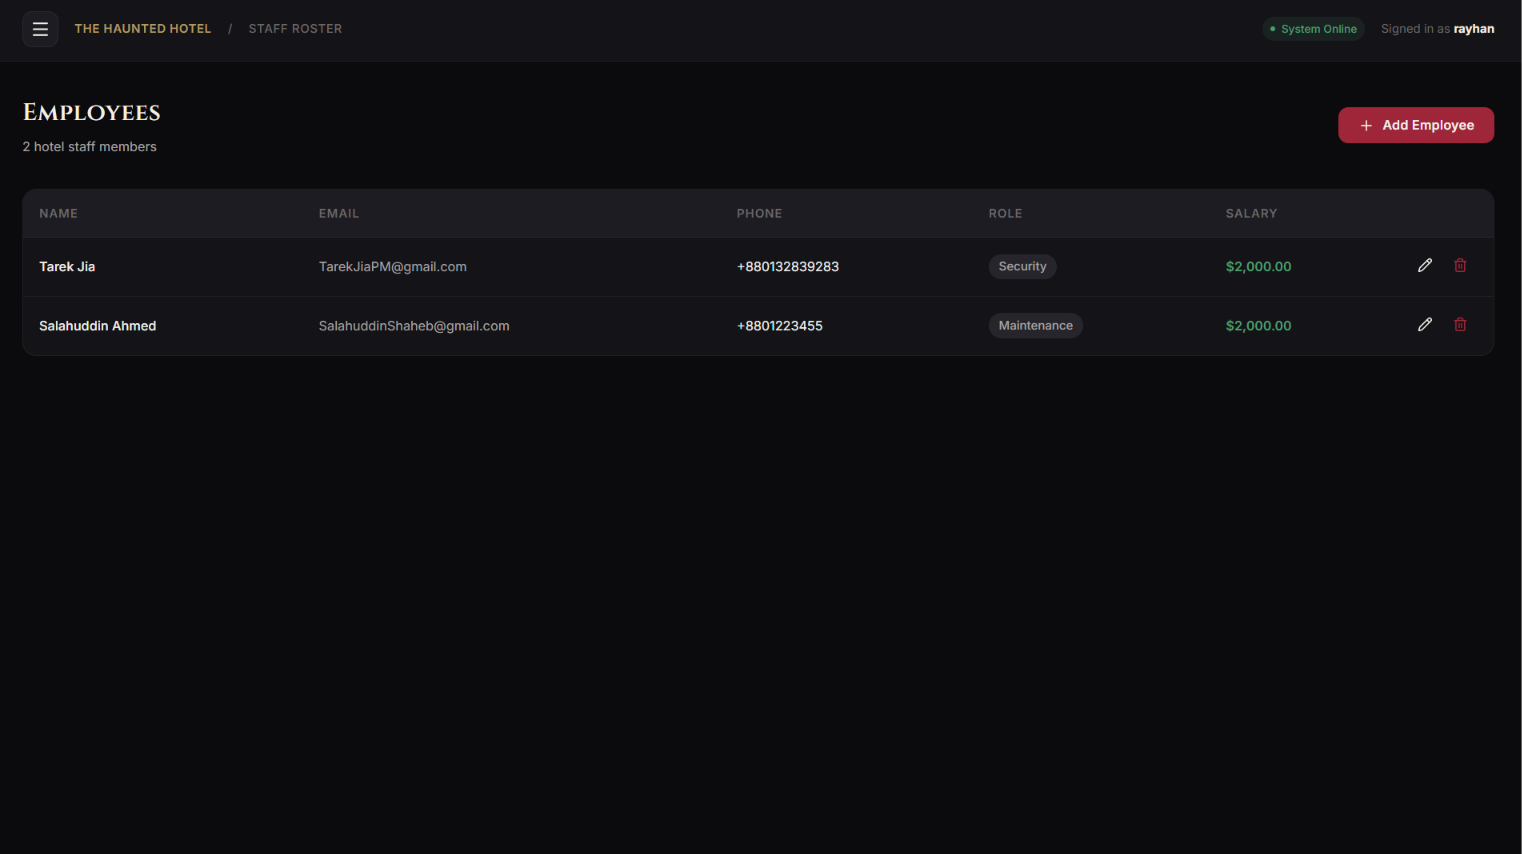
\includegraphics[width=0.92\textwidth]{Employee_Management.png}
}{%
  \IfFileExists{docs/screenshot/Employee_Management.png}{%
    
\includegraphics[width=0.92\textwidth]{docs/screenshot/Employee_Management.png}
  }{%
    \fbox{\parbox{0.9\textwidth}{\centering \vspace{2cm} [Screenshot: Employee Directory Interface] \vspace{2cm}}}
  }
}
\caption{Employee Directory View: Staff Records, Designations, and Monthly Salaries}
\label{fig:ui_emp}
\end{figure}

% =========================================================
% 6. SOFTWARE TESTING
% =========================================================
\section{Software Testing}

\subsection{Testing Methodology and Framework}
Testing was implemented using the \textbf{xUnit} framework alongside the \textbf{Entity Framework Core InMemory provider}. This approach ensures complete test isolation, deterministic repeatability, and fast execution without requiring external database dependencies.

\subsection{Test Suite Breakdown and Results}
\begin{table}[H]
\centering
\caption{Automated Unit and Integration Test Results}
\label{tab:test_results}
\begin{tabularx}{\textwidth}{l X c r}
\toprule
\textbf{Test Category} & \textbf{Primary Assertions Verified} & \textbf{Count} & \textbf{Status} \\
\midrule
Authentication & User creation, BCrypt validation, JWT issuance, duplicate check & 4 & Passed \\
Booking Service & Tariff calculation, overlap detection, state transitions, checkout guard & 10 & Passed \\
Payment Service & Balance calculation, partial payments, overpayment rejection & 8 & Passed \\
Rooms \& Customers & Unique constraint enforcement, search filters, delete restrictions & 8 & Passed \\
Room Availability & Date collision logic, boundary checks, cancellation release & 5 & Passed \\
\midrule
\textbf{Total Suite} & \textbf{Complete Domain and Business Logic Coverage} & \textbf{35} & \textbf{100\% Passed} \\
\bottomrule
\end{tabularx}
\end{table}

% =========================================================
% 7. IMPLEMENTATION AND DEPLOYMENT
% =========================================================
\section{Software Implementation and Deployment}

\subsection{Prerequisites}
\begin{itemize}[leftmargin=*]
  \item \textbf{.NET 10 SDK} for backend compilation and runtime execution.
  \item \textbf{Node.js (v18.0+) and npm} for frontend build bundling and development serving.
  \item \textbf{Microsoft SQL Server} for relational data persistence.
\end{itemize}

\subsection{Execution Instructions}
\begin{lstlisting}[language=bash,caption={Backend Execution Commands}]
# Navigate to API directory and update database schema
cd src/HotelManagement.API
dotnet ef database update --project ../HotelManagement.Infrastructure
dotnet run
# API starts on http://localhost:5048 (Swagger: http://localhost:5048/swagger)
\end{lstlisting}

\begin{lstlisting}[language=bash,caption={Frontend Execution Commands}]
# Navigate to frontend directory and start Vite development server
cd frontend
npm install
npm run dev
# Frontend application opens on http://localhost:5173
\end{lstlisting}

% =========================================================
% 8. CONCLUSION AND FUTURE SCOPES
% =========================================================
\section{Conclusion and Future Scopes}

\subsection{Conclusion}
The Haunted Hotel Management System successfully resolves the operational bottlenecks of traditional hospitality management. By utilizing ASP.NET Core (.NET 10) Clean Architecture, React 19 SPA, Entity Framework Core 9, and Microsoft SQL Server, the system achieves:
\begin{itemize}[leftmargin=*]
  \item Real-time inventory tracking eliminating double bookings.
  \item Server-enforced financial integrity preventing overpayments and arithmetic errors.
  \item Strict role-based authorization securing employee records and payroll.
  \item Visual business intelligence delivering live occupancy rates and revenue metrics.
\end{itemize}

\subsection{Future Scopes}
\begin{itemize}[leftmargin=*]
  \item \textbf{Online Travel Agency (OTA) Channel Integration:} Bidirectional API synchronization with platforms such as Booking.com and Airbnb.
  \item \textbf{Online Payment Gateway Integration:} Direct integration of payment gateways (e.g., Stripe, SSLCommerz, bKash) for automatic customer transactions.
  \item \textbf{Automated Notification Engine:} SMS and email alerts for reservation confirmations and departure invoices.
\end{itemize}

\end{document}
